\documentclass{beamer}
\usepackage{times}
\usepackage{tikz}
\usepackage{beamerthemesplit}
\usepackage{tcolorbox}

\title{The Security Framework of White-Box Cryptography Revisited}
\author{scnucrypto\inst{1,2}\\ \url{cis.gong@gmail.com}}
\institute{\inst{1}{School of Computer Science, South China Normal University} \\ \inst{2}{Mobile Applications And Security Engineering Center of Guangdong Province}}

\date{\today}

\begin{document}

\frame
{
 \titlepage
}

\section[Outline]{}
\frame{\tableofcontents}

\section{White-box cryptography: background}
\frame{
\frametitle{Cryptography: the very beginning}
"Information theory is about communication in the presence of noise."
\begin{flushright}
-C. Shannon, 1948.\footnote{\scriptsize{\url{http://fab.cba.mit.edu/classes/S62.12/docs/Shannon_noise.pdf}}}
\end{flushright}

\begin{center}
\begin{tikzpicture}
    \node[anchor=south west,inner sep=0] (image) at (0,0) { 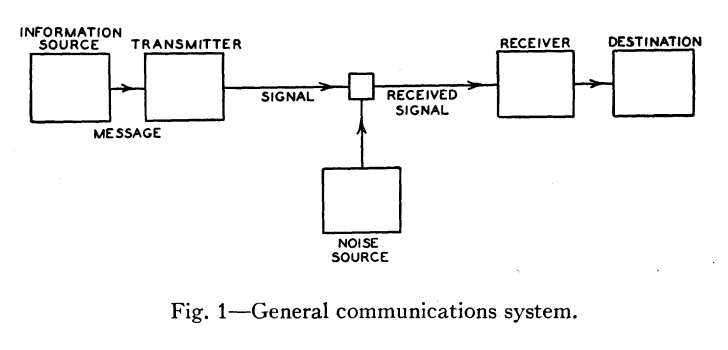
\includegraphics[width=8cm, height=4cm]{./pics/Shannon_GeneralCommunicationSystem.png}};

    %\begin{scope}[x={(image.south east)},y={(image.north west)}]
        %\draw[help lines,xstep=.1,ystep=.1] (0,0) grid (1,1);
        %\foreach \x in {0,1,...,9} { \node [anchor=north] at (\x/10,0) {0.\x}; }
        %\foreach \y in {0,1,...,9} { \node [anchor=east] at (0,\y/10) {0.\y}; }
        %\draw[green, ultra thick, rounded corners] (0.24,0.18) rectangle (0.50,0.32);
    %\end{scope}
\end{tikzpicture}
\end{center}
}

\frame{
\frametitle{Cryptography: an informal definition}
"Cryptography is about communication in the presence of adversaries."
\begin{flushright}
-R. Rivest
\end{flushright}

\begin{center}
\begin{tikzpicture}
    \node[anchor=south west,inner sep=0] (image) at (0,0) { 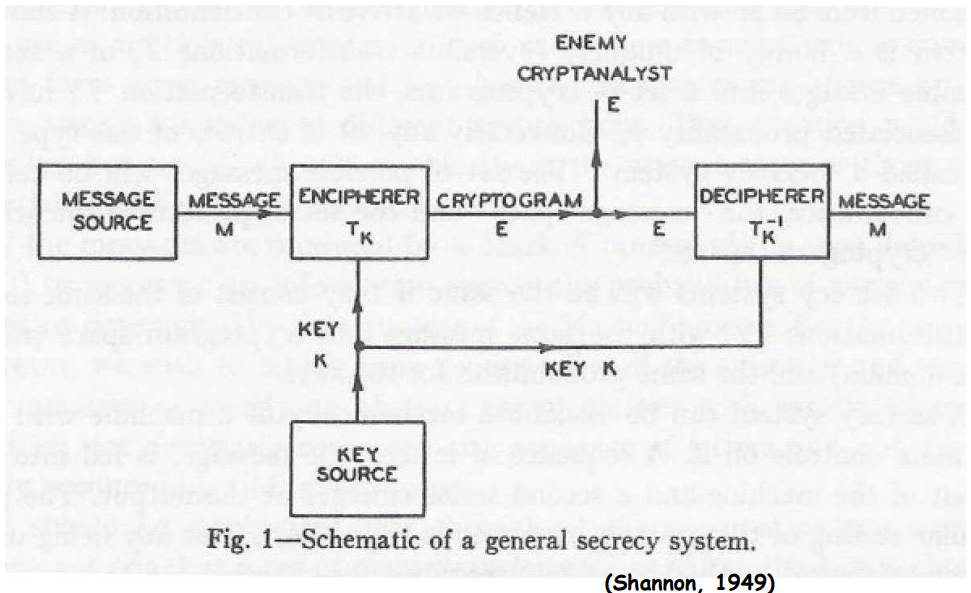
\includegraphics[width=8cm, height=5cm]{./pics/Shannon_GeneralSecrecySystem.png}};

    %\begin{scope}[x={(image.south east)},y={(image.north west)}]
        %\draw[help lines,xstep=.1,ystep=.1] (0,0) grid (1,1);
        %\foreach \x in {0,1,...,9} { \node [anchor=north] at (\x/10,0) {0.\x}; }
        %\foreach \y in {0,1,...,9} { \node [anchor=east] at (0,\y/10) {0.\y}; }
        %\draw[green, ultra thick, rounded corners] (0.24,0.18) rectangle (0.50,0.32);
    %\end{scope}
\end{tikzpicture}
\end{center}
}

\frame{
\frametitle{Define a secrecy system in ``a mathematically acceptable way"}
\textcolor{red}{``As a first step in the mathematical analysis of cryptography, it is necessary to idealize the situation suitably, and to define in a mathematically acceptable way what we shall mean by a secrecy system."}

\begin{flushright}
-C. Shannon, 1949. \footnote{{\scriptsize``Communication Theory of Secrecy Systems", Bell System Tech. J., vol. 28, pp. 656-715, Oct., 1949.}}
\end{flushright}
}

\frame{
\frametitle{The Kerckhoffs' principle of a secrecy system}
A cipher should be secure when the enemy cryptanalyst knows all details of the enciphering process and deciphering process except for the value of the secret key.

\begin{flushright}
- stated in 1881 by the Dutchman Auguste Kerckhoffs (1835-1903).
\end{flushright}


\begin{center}
\begin{tikzpicture}
    \node[anchor=south west,inner sep=0] (image) at (0,0) { 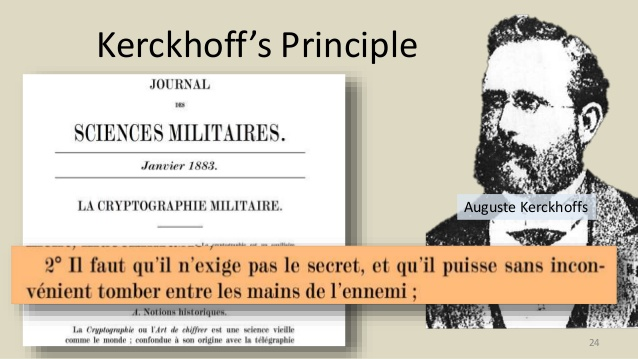
\includegraphics[width=6cm, height=4cm]{./pics/Kerckhoffs.jpg}};

    %\begin{scope}[x={(image.south east)},y={(image.north west)}]
        %\draw[help lines,xstep=.1,ystep=.1] (0,0) grid (1,1);
        %\foreach \x in {0,1,...,9} { \node [anchor=north] at (\x/10,0) {0.\x}; }
        %\foreach \y in {0,1,...,9} { \node [anchor=east] at (0,\y/10) {0.\y}; }
        %\draw[green, ultra thick, rounded corners] (0.24,0.18) rectangle (0.50,0.32);
    %\end{scope}
\end{tikzpicture}
\end{center}
}

\frame{
\frametitle{The goal of modern cryptography}
To my opinion, the goal of modern cryptography is to design, analysis, and implement a secrecy system which obtains a mathematically acceptable security proofs.

\begin{itemize}
\item Confidentiality / Secrecy
\item Integrity
\item Authenticity
\item Availability
\end{itemize}
}

\frame{
\frametitle{White-box model}
\begin{itemize}
\item Informally speaking, an adversary in \textcolor{red}{white-box model} can tamper, modify, manipulate all intermediate values and processes of the implementation of a secrecy system.
\item It can be looked as a superset of \textcolor{red}{black-box} and \textcolor{red}{grey-box} models.
\end{itemize}

\begin{center}
\begin{tikzpicture}
    \node[anchor=south west,inner sep=0] (image) at (0,0) { 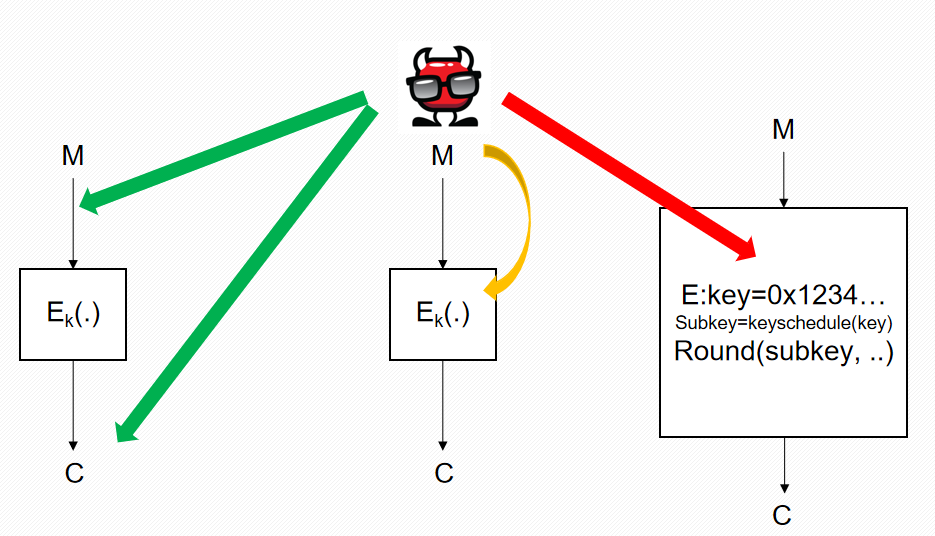
\includegraphics[width=7cm, height=4cm]{./pics/WBC_Model.png}};

    %\begin{scope}[x={(image.south east)},y={(image.north west)}]
        %\draw[help lines,xstep=.1,ystep=.1] (0,0) grid (1,1);
        %\foreach \x in {0,1,...,9} { \node [anchor=north] at (\x/10,0) {0.\x}; }
        %\foreach \y in {0,1,...,9} { \node [anchor=east] at (0,\y/10) {0.\y}; }
        %\draw[green, ultra thick, rounded corners] (0.24,0.18) rectangle (0.50,0.32);
    %\end{scope}
\end{tikzpicture}
\end{center}
}

\section{White-box cryptography: basic concepts}


\end{document}